Während in Mariposa vier Schlösser für unsere Unversehrtheit sorgten, übernahm dies in \TOWN{Three Lakes} ein indisches Gebet.
Es gab mal wieder ein Frühstück, das aus Toast, Kuchen, Cornflakes und Waffeln bestand.
Besteck war aus Plastik, ebenso die Teller und am Schluss landete alles im Müll.
Man aß quasi Müll von Müll mit Müll.

Im Yosemite National Park gab es einzelne Flecken an denen Sequoias wachsen, aber es gibt auch einen eigenen Sequoia National Park.
Der war unser heutiges Vormittagsprogramm.
Und dort ist es dann passiert!
Dem Christian waren die Jungs auf den ersten Blick wieder nicht koscher genug, aber ich saß am Steuer und so hielten wir an.
Räumten die Rücksitzbank auf und die Herren waren an Bord.
Neusseländer hatten wir da aufgegabelt, die mit ihrem Wohnmobil nicht bis hoch zu den Sequoias fahren konnten.
Sie waren in den USA, da sie eine Firma betreiben um mit Drohnen zu filmen.
Dafür erhielten sie einen Preis und machten danach noch Urlaub.
Am Informationszentrum trennten sich die Wege wieder, wir lasen uns schlau und wer hätte es gedacht, die Amis räumen doch glatt ein, dass sie in der Vergangenheit ganz falsch mit den Sequoias umgegangen sind.
Unter anderem gab es an Ort und Stelle mal eine Tankstelle und durch das Löschen von Waldbränden kamen auch keine neuen Sequoias hinzu.

\newpage
\thispagestyle{empty}
\begin{tikzpicture}[remember picture, overlay]
\node[inner sep=0pt] at (current page.center) {%
	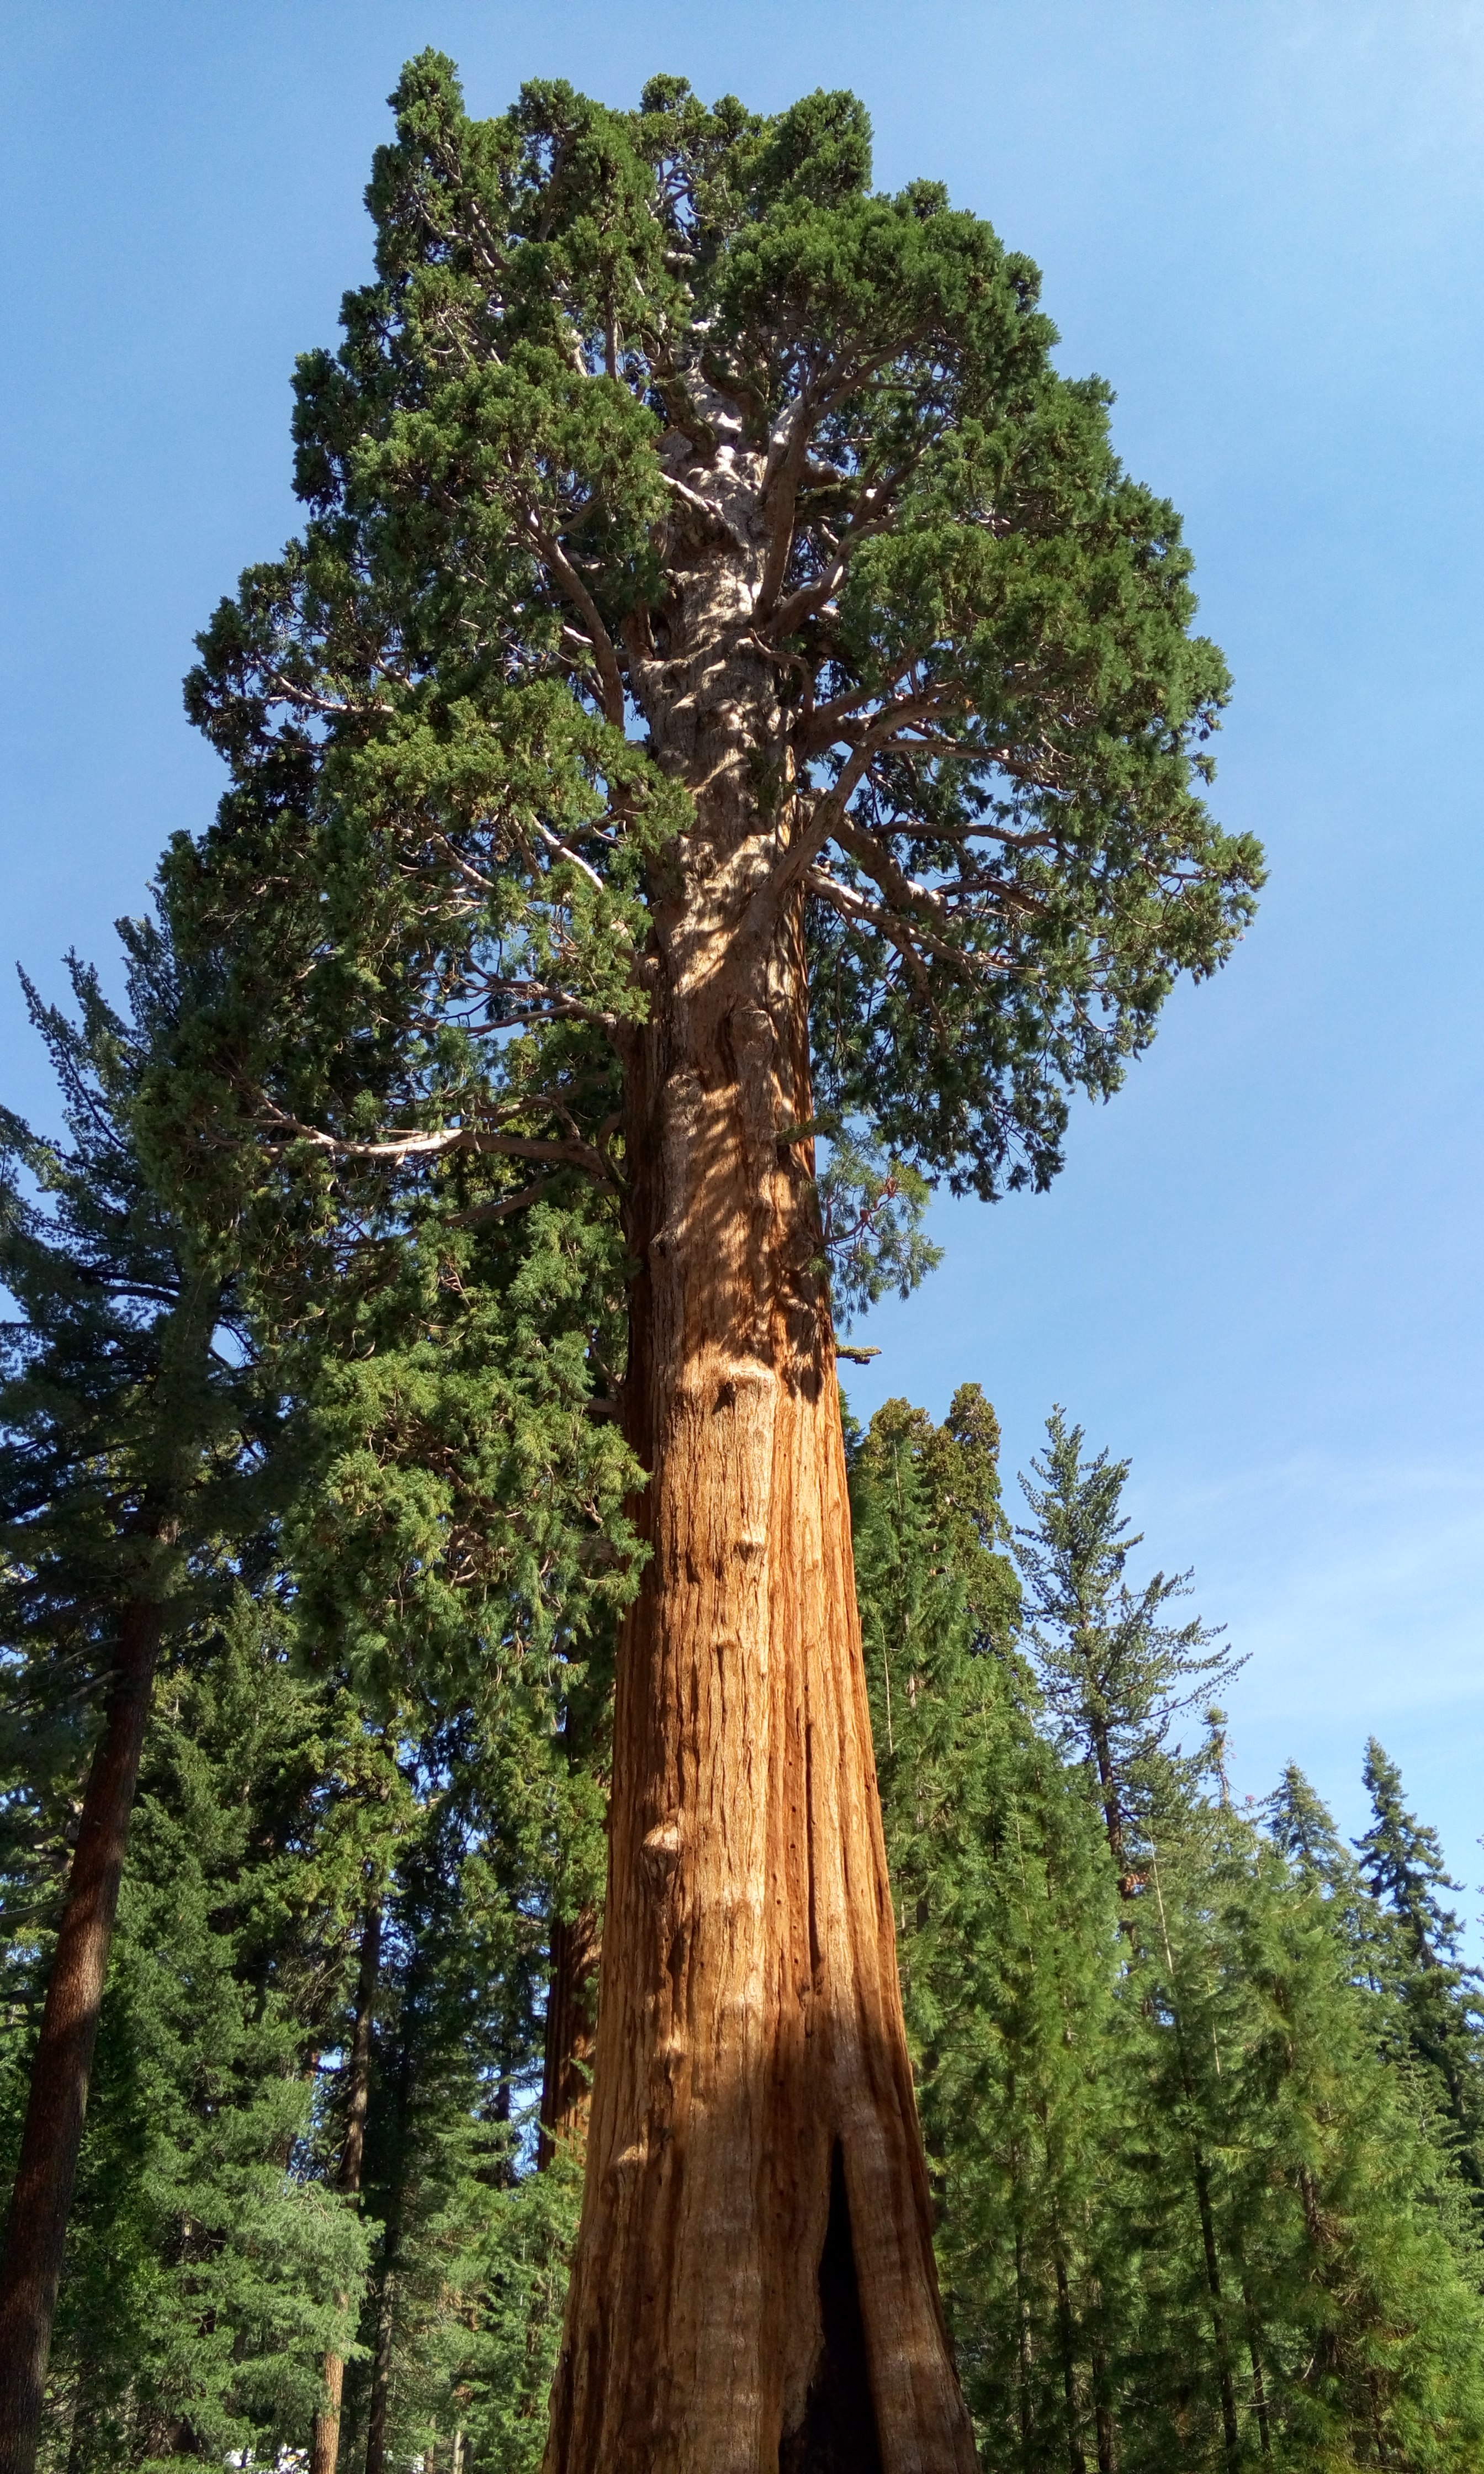
\includegraphics[angle=0,width=\paperwidth,height=\paperheight]{26/image20160426_101234649.jpg};%
};
\end{tikzpicture}
\newpage

Nachdem wir genug große Bäume gesehen hatten, fuhren wir weiter zum \TOWN{Death Valley}.
500~km dürften es locker gewesen sein.
Da unser Bett für die Nacht jedoch auf der anderen Seite lag, fuhren wir gleich mal durch.
Ein gewisser Nervenkitzel war dabei, der Tankinhalt war recht überschaubar und im \TOWN{Death Valley} gibt es nur eine einzige Tankstelle mit sehr überteuerten Preisen.

Angekommen sind wir und die Tankstelle in \TOWN{Beatty} hatte auch wieder bessere Preise.
Da wir die Pizza für \glqq take-away \grqq bestellen wollten, haben wir auch keine I.D mitgenommen.
Leider dauerte es 30~m bis die Pizza fertig war und die nette Bedienung bot uns derweil ein Bier an obwohl wir keine I.D hatten.
Die Pizza war gut sowie das Helle!
